\section{Module Overview}

\subsection{Module List}
The project codebase is divided into the following components with the corresponding responsibilities.

\begin{itemize}
    \item \textbf{driver} - The main driver of the codebase that is responsible for driving the entire callgraph generation process. It is the only public interface. It contains the longest running function throughout the process.
    \item \textbf{lib-frontend} - This library contains the parser and lexer that takes Javascript source code converts it to an ESTree\parencite{estree} compliant Abstract Syntax Tree. It performs other tasks such as tweaking the Abstract Syntax Tree to annotate enclosing files and functions. 
    \item \textbf{lib-ir} - This library generates symbol tables that behave like hashmaps to store the scopes that variables and functions occur in.
    \item \textbf{lib-callgraph} - This library is in charge of generating the callgraph and flowgraph, which are the output facts that we require.
\end{itemize}

\subsection{Dependency Structure}

The diagram below shows the dependencies between the various modules. \textbf{driver} is in charge of calling functions from the various modules. In turn, they all rely on various utility functions from the \textbf{utils} module.

\begin{center}
    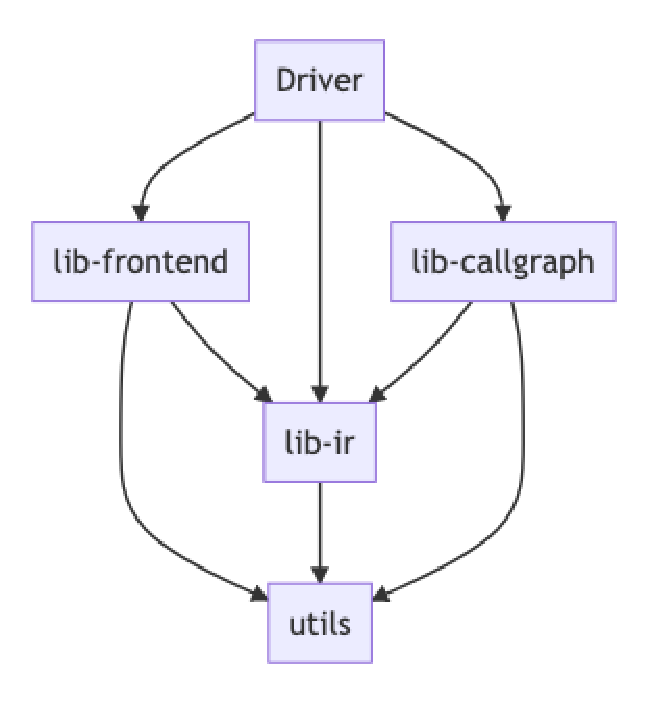
\includegraphics[height=300pt]{./images/dependency.eps}
\end{center}
